\section{Results}
\subsection{Key Observations}
\begin{itemize}
    \item \textbf{Persistence of Quantum Coherence:} Simulations revealed that microtubules maintain coherence for extended durations, even under external influences of decoherence. This challenges assumptions of rapid decoherence in biological systems and supports the hypothesis of intrinsic quantum stabilization mechanisms.
    \item \textbf{Fibonacci Scaling as a Stabilizing Factor:} Incorporating Fibonacci scaling into the models demonstrated resonance patterns that reduce wave packet dispersion and conserve coherence, suggesting a fundamental role for universal mathematical principles in biological quantum systems.
    \item \textbf{Event Horizon Analogies:} Cytokine-induced decoherence simulations revealed localized boundary-like behaviors analogous to astrophysical event horizons, suggesting that microtubules may possess quantum boundaries that protect coherence.
\end{itemize}

\subsection{Visualization of Quantum Event Horizon-like Boundaries}
\begin{figure}[H]
    \centering
    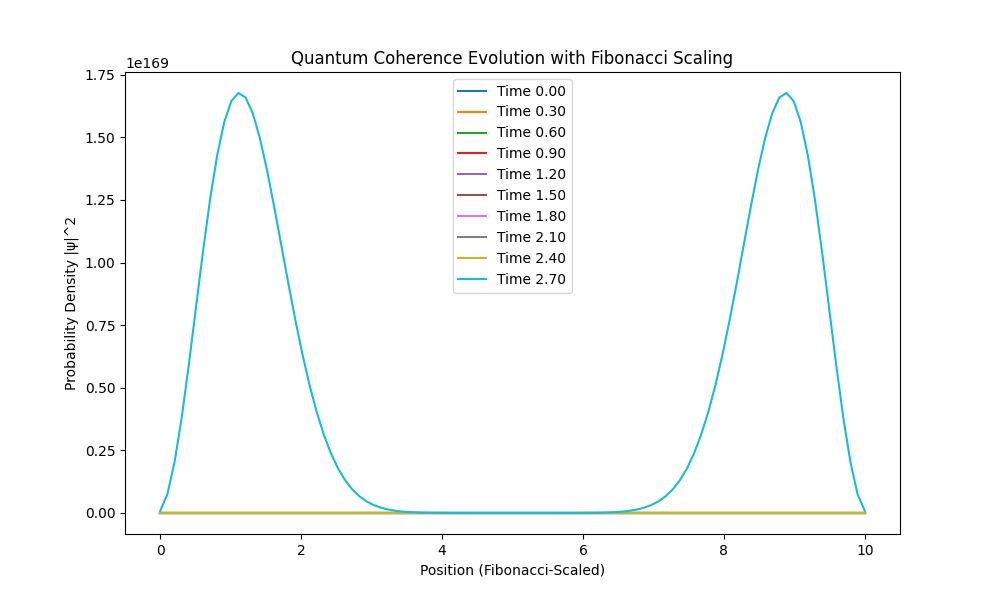
\includegraphics[width=0.8\textwidth]{Microtubule_Simulation/figures/quantum_coherence_evolution.png}
    \caption{1D Simulation of Gaussian Wave Packet Dynamics. Persistent peaks at boundary regions indicate the presence of event horizon-like quantum sanctuaries. These results suggest that microtubules may form coherence-protecting zones, analogous to event horizons in astrophysics.}
    \label{fig:event_horizon}
\end{figure}

\subsection{Fibonacci Scaling in Microtubules}
\begin{figure}[H]
    \centering
    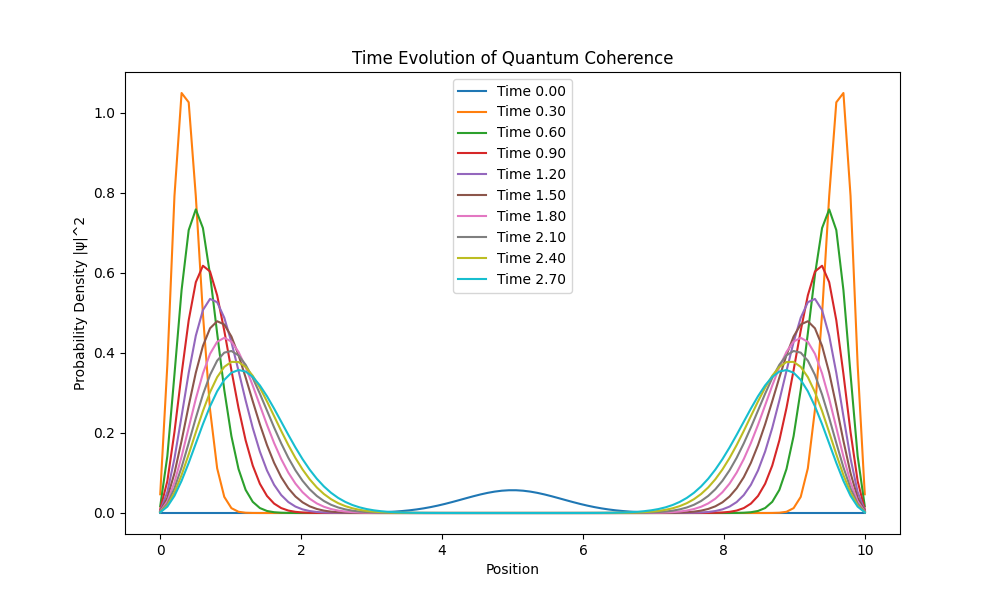
\includegraphics[width=0.75\textwidth]{Microtubule_Simulation/figures/fibonacci_wavefunction_evolution.png}
    \caption{Time-evolved probability density showing the stabilization of quantum coherence under Fibonacci scaling. The recursive structure of Fibonacci scaling appears to reduce wave packet dispersion, potentially acting as a fundamental stabilizing factor in biological quantum systems.}
    \label{fig:fibonacci_scaling}
\end{figure}

\subsection{2D Wavefunction Probability Density}
\begin{figure}[H]
    \centering
    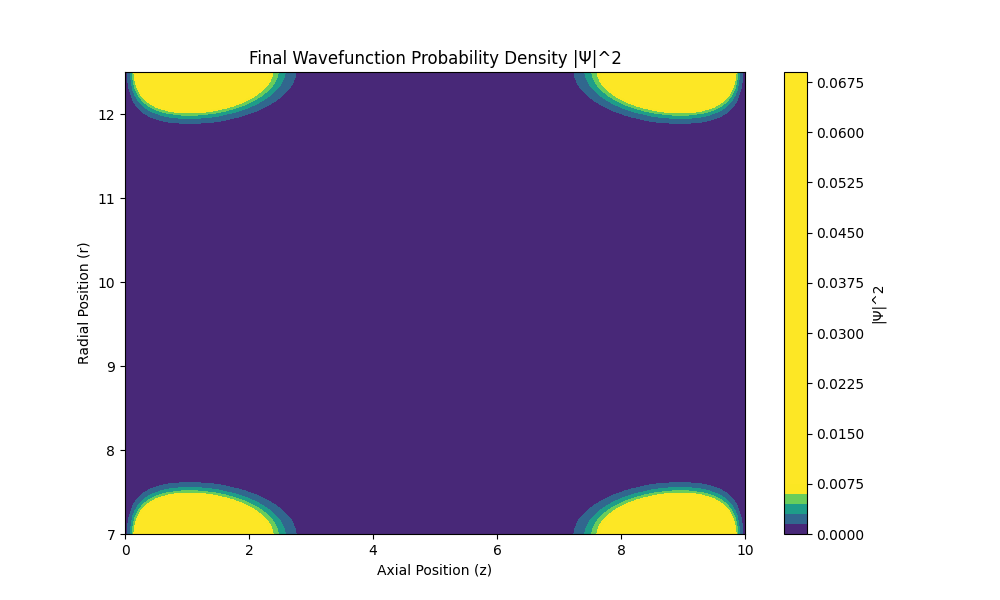
\includegraphics[width=0.8\textwidth]{Microtubule_Simulation/figures/wavefunction_probability_density.png}
    \caption{2D probability density distribution of the quantum wavefunction in microtubules. Bright regions represent areas of prolonged coherence, demonstrating how Fibonacci scaling influences wavefunction behavior in two dimensions.}
    \label{fig:wavefunction_2D}
\end{figure}

\subsection{2D Plots in Cylindrical Geometry}
\begin{figure}[H]
    \centering
    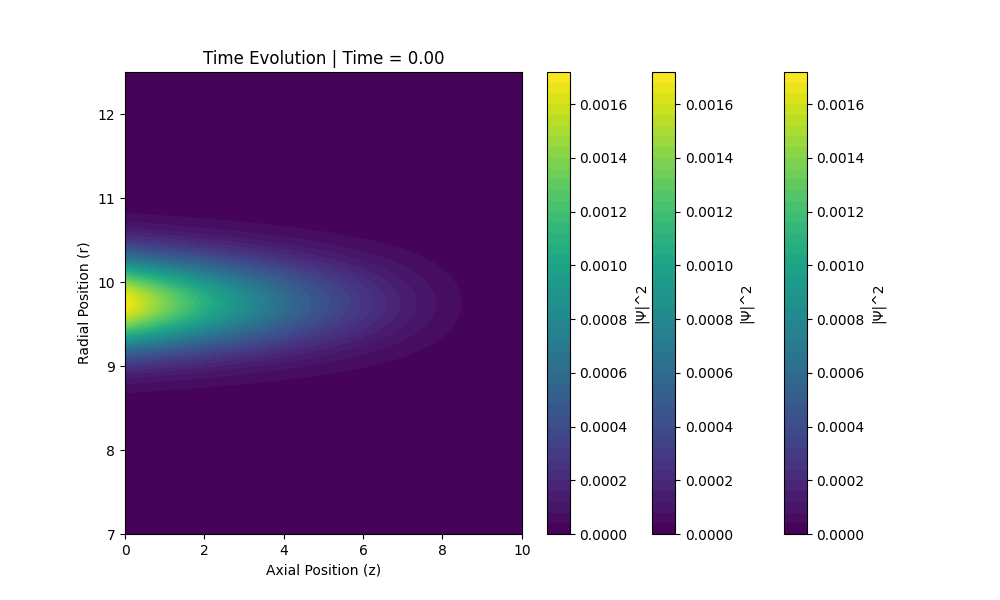
\includegraphics[width=0.8\textwidth]{Microtubule_Simulation/figures/cylindrical_evo0.png}
    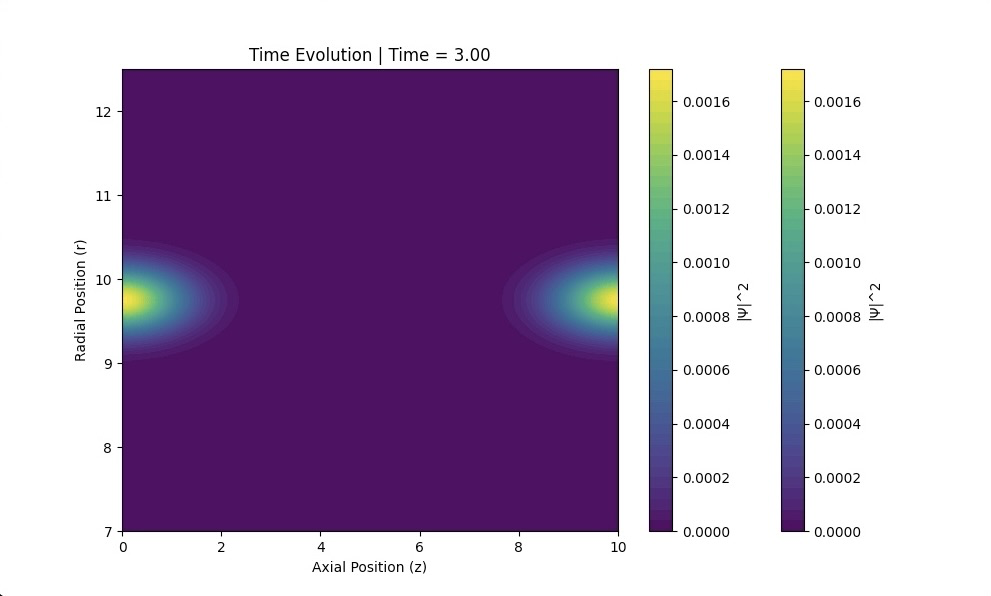
\includegraphics[width=0.8\textwidth]{Microtubule_Simulation/figures/cylindrical_evo3.png}
    \caption{Time evolution of the wavefunction in cylindrical microtubule geometry. The top panel shows the initial state, while the bottom panel illustrates the evolved wavefunction over time. This visualization supports the hypothesis that coherence may be preserved through structural constraints in microtubules.}
    \label{fig:cylindrical_geometry}
\end{figure}
\FloatBarrier  % Ensures all figures appear before the next section starts 

\begin{figure}[H]
    \centering
    \includegraphics[width=0.8\textwidth]{Microtubule_Simulation/figures/ultra_light_code_enhancements.png}
    \caption{Final high-resolution simulation of coherence evolution in HAND. Early HAND shows minor coherence loss, while late-stage HAND exhibits severe collapse due to viral toxicity.} \label{fig:HIV_coherence_evolution_final}
\end{figure}

\begin{figure}[H]
    \centering
    \includegraphics[width=0.8\textwidth]{Microtubule_Simulation/figures/ultra_light_false.png}
    \caption{Comparative coherence degradation across different stages of HIV infection. Uncontrolled HIV results in widespread coherence collapse, whereas ART-controlled HIV retains partial coherence but remains vulnerable to stochastic cytokine fluctuations.}
    \label{fig:HIV_coherence_stages}
\end{figure}

%\begin{figure}[H]
%\centering
%\includegraphics[width=0.8\textwidth]{Microtubule_Simulation/figures/Graphic_abstract_final550_1100.png}
 %   \caption{Graphical abstract summarizing the study. Quantum coherence is initially stable in microtubules, but cytokine-induced perturbations lead to progressive coherence loss, culminating in structural collapse in late-stage HAND.}
 %   \label{fig:HIV_graphical_abstract}
%\end{figure}
\FloatBarrier  % Ensures all figures appear before the next section starts
